\section{Experiment}

\subsection{System Parameter}
The threshold is the only adjusted parameter in the system.
We use three thresholds to represent different risk preferences.  
\begin{table}[htb]
    \centering
    \begin{tabular}{||c|c||}
    \hline \hline
    Threshold $\theta$ & Risk Preference \\ \hline
    No plenty ($\infty$) & High \\ \hline
    0.006 & Medium      \\ \hline
    0.002 & Low      \\ \hline \hline
    \end{tabular}
    \caption{Threshold and Risk Preferences}
    \label{tab:threshold}
\end{table}
\subsection{Trading Frequency}
Our trading frequency is weekly. Compare to trading daily, reducing the trading frequency will reduce the impact of trading fees and slippage.

\subsection{Validation Period}
To verify the robustness of our system, we validate our system on two validation periods with different characteristics. Both validation periods have at least on significant decline period to prove our system regulates MDD.
\begin{table}[htb]
    \centering
    \begin{tabular}{||c|c|c|c|c||}
    \hline \hline
    \multirow{2}{*}{Period} &
    \multirow{2}{*}{Start} &
    \multirow{2}{*}{End} &
    \multicolumn{2}{c||}{S\&P 500} \\ 
    \cline{4-5} &{} &{} & CAGR & MDD \\ \hline \hline
    Period 1 & 2017/3/1 & 2019/2/28 & 7.81\% & 19.78\% \\ \hline
    Period 2 & 2019/3/1 & 2021/3/15 & 18.56\% & 33.9\% \\    
    \hline \hline
    \end{tabular}
    \caption{Validation Period}
    \label{tab:validation_period}
\end{table}
\begin{figure}[htb]
    \centering
    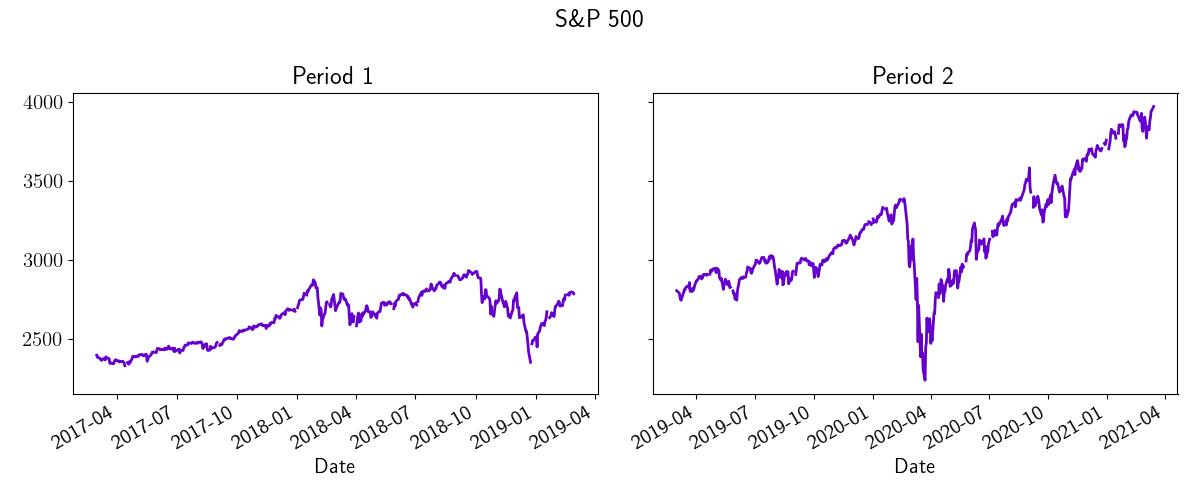
\includegraphics[width=15cm]{images/sp500.png}
    \caption{S\&P 500 of validation period}
    \label{fig:my_label}
\end{figure}

\subsection{Baseline}
A Constant rebalanced portfolio (CRP) is an investment strategy that keeps a constant ratio between all investments over time. We use this to represent the portfolio provided by advisors to meet investors' risk preferences. We will use the average ratio of our portfolio to build a CRP portfolio and use it as a baseline for performance comparison in MDD and CAGR.
\subsection{Result}
Our system successfully delivers portfolios with different MDD to meet various investors' preferences, and output performed CRP in MDD and CAGR in most situations.





\begin{figure}[htb]
\centering
  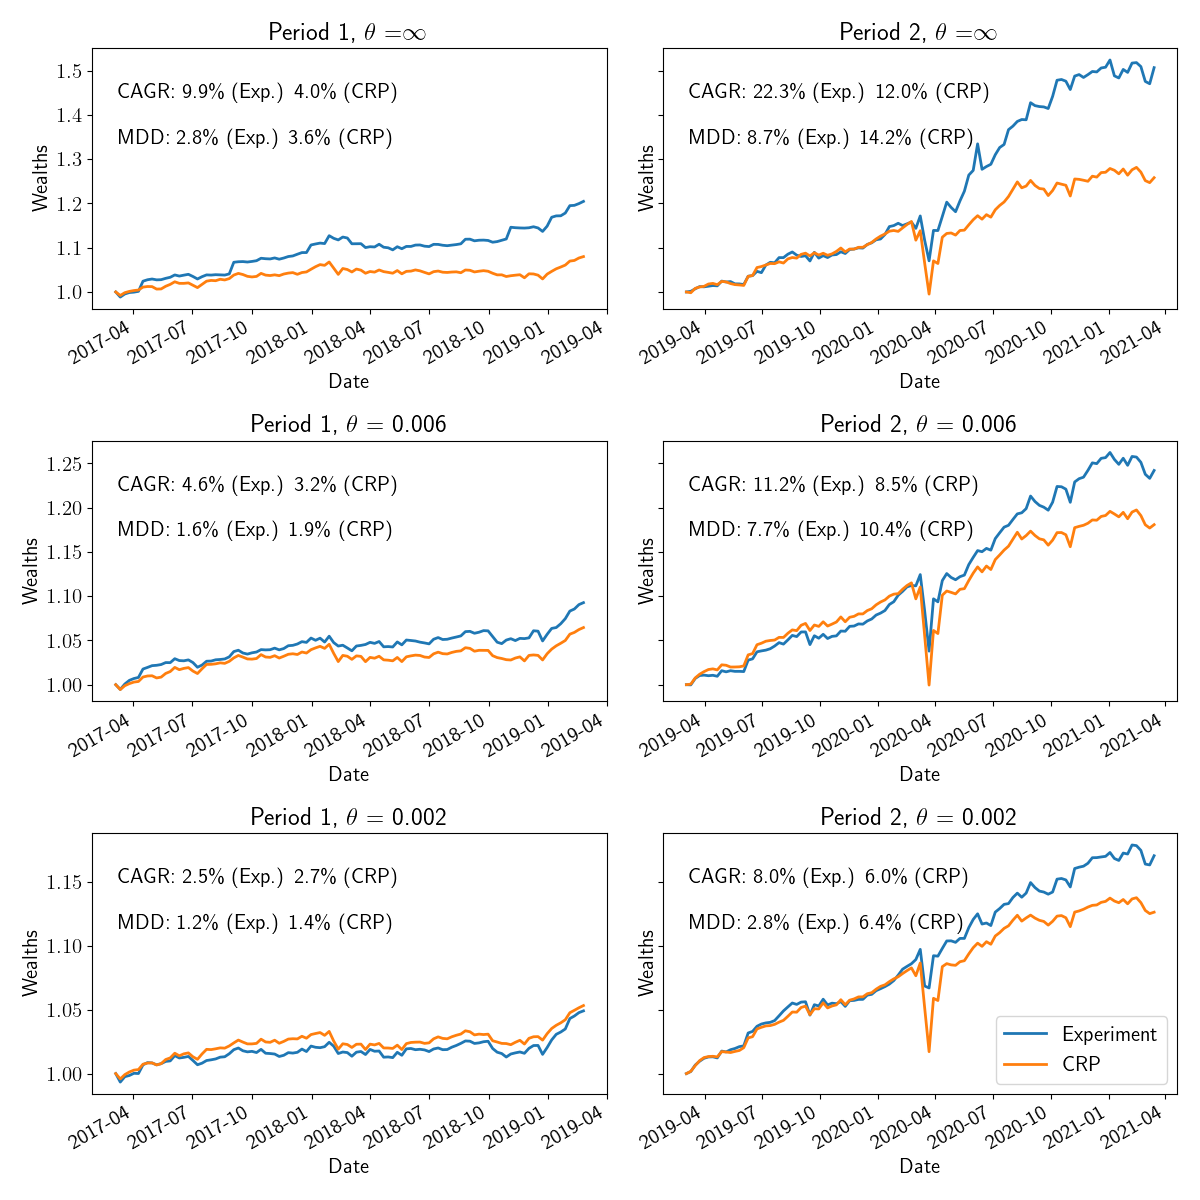
\includegraphics[width=16cm]{images/crp_compare.png}
  \caption [Comparison of experiments result with CRP]{Comparison of experiments result with CRP}
  \label{fig:crp_compare}
\end{figure}

\par
SPY is the investment with high risk among our investment universe. After a deep dive into the portfolios, we observed portfolios with different risk preferences, adjusted by $\theta$, contain different SPY weights. The portfolio with high-risk preference contains more weight on SPY than the portfolio for low-risk preference.
\begin{figure}[htb]
\centering
  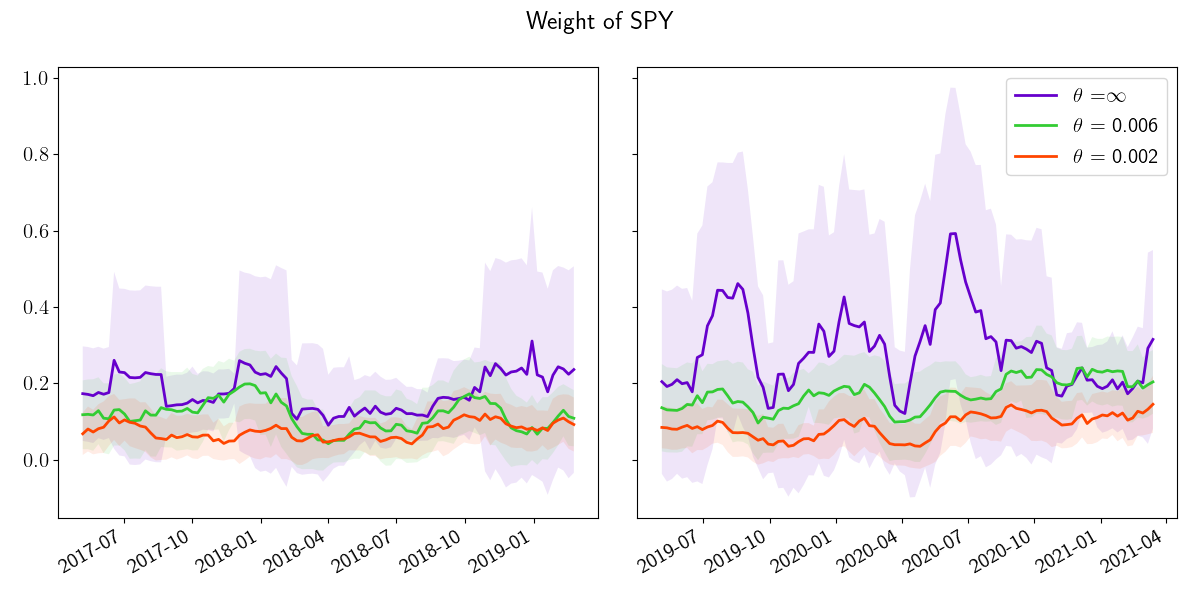
\includegraphics[width=16cm]{images/spy_weight.png}
  \caption [Comparison of portfolio in term of weight of SPY]{Comparison of portfolio in term of weight of SPY in the portfolio, moving average 70 days.The portfolio for high-risk preference contains more weight on SPY than the portfolio for low-risk preference.
  }
  \label{fig:crp_compare}
\end{figure}